%%%%%%%%%%%%%%%%%%%%%%%%%%%%%%%%%%%%%%%%%
% a0poster Portrait Poster for LiRI/UZH
% LaTeX Template
% Version 1.0 (22/06/13)
% Version 2.0 (08/04/22)
%
% The a0poster class was created by:
% Gerlinde Kettl and Matthias Weiser (tex@kettl.de)
% adapted by Danny McDonald for LiRI/UZH (mcddjx@gmail.com)
%
% License:
% CC BY-NC-SA 3.0 (http://creativecommons.org/licenses/by-nc-sa/3.0/)
%
%%%%%%%%%%%%%%%%%%%%%%%%%%%%%%%%%%%%%%%%%

\documentclass[a0,portrait]{a0poster}

% control margins here
\usepackage{geometry}
 \geometry{
 a0paper,
 left=5cm,
 top=4.5cm,
 right=5cm,
 bottom=4.5cm
 }
\addtolength{\textwidth}{4.5cm} % width of text can be adjusted if margins above are adjusted
\usepackage{float}
\usepackage{smartdiagram}
\usepackage{metalogo}
\usepackage{dtklogos}
\usepackage{multicol} % This is so we can have multiple columns of text side-by-side
\columnsep=3em % This is the amount of white space between the columns in the poster
\columnseprule=0pt % This is the thickness of the black line between the columns in the poster
\usepackage{dirtree}
\usepackage{hyperref}
% UZH colours
\usepackage{multirow}
\usepackage{tikz}
\usetikzlibrary{shapes}
\usetikzlibrary{arrows}
% Define block styles
\tikzstyle{decision} = [diamond, draw, fill=blue!20, 
    text width=4.5em, text badly centered, node distance=3cm, inner sep=0pt]
\tikzstyle{block} = [rectangle, draw, fill=blue!20, 
    text width=5em, text centered, rounded corners, minimum height=4em]
\tikzstyle{line} = [draw, -latex']
\tikzstyle{cloud} = [draw, ellipse,fill=red!20, node distance=3cm,
    minimum height=2em]

\definecolor{uzhblau100}{RGB}{0,40,165}
\definecolor{Black}{RGB}{0,0,0}
\definecolor{uzhblau80}{RGB}{51,83,183}
\definecolor{uzhockerrot100}{RGB}{220, 96, 39}
\definecolor{uzhockerrot80}{RGB}{227, 128, 82}
\definecolor{uzhflaschengruen100}{RGB}{42, 127, 98}
\definecolor{uzhflaschengruen80}{RGB}{86, 157, 133}
\definecolor{conclusion}{RGB}{204,212,237} % the conclusion box colour
\definecolor{binanceyellow}{RGB}{243, 186, 47}
\usepackage{ifthen} % needed to stop horizontal line above 'Conclusions' section
\usepackage{graphicx} % Required for including images
\graphicspath{{figures/}} % Location of the graphics files
\usepackage{mwe,tikz}\usepackage[percent]{overpic} % overlay your photo over the background
\usepackage{booktabs} % Top and bottom rules for table
\usepackage[font=small,labelfont=bf]{caption} % Required for specifying captions to tables and figures
\usepackage{amsfonts, amsmath, amsthm, amssymb} % For math fonts, symbols and environments
\usepackage{wrapfig} % Allows wrapping text around tables and figures

\usepackage{fontspec} % custom fonts
\defaultfontfeatures[Palatino]
{
    Extension = .ttf,
    UprightFont = font/LT_41167,
    BoldFont = font/LT_41169,
    ItalicFont  = font/LT_41168,
    BoldItalicFont = font/LT_41170,
}
\defaultfontfeatures[TheSans]
{
    Extension = .otf,
    UprightFont = font/TheSans-LP5Plain,
    BoldFont = font/TheSans-LP7Bld,
    ItalicFont  = font/TheSans-LP5PlainIT,
    BoldItalicFont = font/TheSans-LP7BldIT,
}
\setmainfont{TheSans} % choose your font here
\usepackage[onehalfspacing]{setspace} % remove for single spacing
\usepackage{tcolorbox} % for the conclusions box
\usepackage{blindtext} % you can remove this once you add your content
\usepackage[export]{adjustbox} % allow floating a graphic right
\usepackage{titlesec} % customising section titles
\usepackage{needspace} % prevent break between line and section title
\usepackage{nameref} % package and command to get the name of the current section (for ifthen)

\begin{document}

% define how our section titles will look (with ruled line)
\titleformat{\section}
  {\needspace{0\baselineskip}\sectionrule\huge\bfseries}
  {\color{Black}\thesection.}
  {1em}
  {\color{Black}}

% draw horizontal line before section unless it is conclusions (if you change name of Conclusions, you should
% also change it here too so it is recognised and the line suppressed
\makeatletter
\newcommand{\sectionrule}{%
 \ifthenelse{\equal{\@currentlabelname}{Conclusions}}
 % use the below line instead of the above if conclusions is a section*
 % \ifthenelse{\equal{\@currentlabelname}{}}
  {}
  {\vspace*{-\baselineskip}
   \vrule height 1pt depth 1pt width \linewidth\vskip0.4pt
   \bigskip}%
}
\makeatother


%----------------------------------------------------------------------------------------
%   POSTER HEADER 
%----------------------------------------------------------------------------------------
%\title{Creating a \LaTeX{} poster template matching UZH specifications for LiRI presentations}
\title{Intern Program Presention}

% the top logo (in english!) and unit title
\noindent
\begin{minipage}{.32\linewidth}
 
\includegraphics[width=20cm]{Binancecompanylogo.png}
\end{minipage}%
\begin{minipage}{.33\linewidth}
 \huge{\textbf{Security \& IT\\(Smart Contract Security)}}
\end{minipage}
\vspace{4em}

% The header is divided into two boxes, on the left is the text and on the right is the image
\begin{minipage}[b][][t]{.3\linewidth}
\vfill
\makeatletter
\raggedright{\fontsize{92pt}{100pt}\selectfont\color{binanceyellow}\textbf{{\@title}}\par}
\makeatother
\color{Black}
\vspace{1cm}
%\Huge\textit{Subtitle goes here}\\[2.4cm] % Subtitle if it exists
\LARGE\underline{Mu Changrui}@Binance\\
\vspace{0.2cm}
\large \textbf{Education Background}:\\
\large
* Bachelor of Computing (Information Security) (Top5\%)      - NUS
%\\ % add your institution
%\texttt{you@uzh.ch}%\\ % add your email
\end{minipage}%
%
\begin{minipage}[b][][t]{.3\linewidth}
\vfill
\large \textbf{Pre-Experience}:\\
\large
* Backend  Engineer Intern                                  - TikTok\\
* Research Assistant on Cryptography                - NUS
  %\begin{overpic}[width=.8\textwidth,right]{LIRI_WissPoster_Wasserzeichen.png} % what even is this thing?
   %  \put(85,0){\includegraphics[scale=0.25]{Silhouette.png}}  % your image goes in here
  %\end{overpic}
\end{minipage}
\vspace{0cm}
\begin{minipage}[b][][t]{.4\linewidth}
\vfill
\large \textbf{Reward:}\\
\large
* 2nd Place in Singapore Blockchain Innovation Challenge 2021   - SBIP\\
* Dean’s List (2020-2021)                               - NUS\\
* Top Student in Computer Security                      - NUS
  %\begin{overpic}[width=.8\textwidth,right]{LIRI_WissPoster_Wasserzeichen.png} % what even is this thing?
   %  \put(85,0){\includegraphics[scale=0.25]{Silhouette.png}}  % your image goes in here
  %\end{overpic}
\end{minipage}
\vspace{0cm}

%----------------------------------------------------------------------------------------
%   POSTER BODY
%----------------------------------------------------------------------------------------

\begin{multicols}{2} % This is how many columns your poster will be broken into

%----------------------------------------------------------------------------------------
%   INTRODUCTION
%----------------------------------------------------------------------------------------

\section{Smart Contract Security Team}
\large
\begin{table}[H]
\centering
\begin{tabular}{|c|c|}
\hline
\multirow{4}{*}{\textbf{Tool Development}} & Code Audit                    \\ \cline{2-2} 
                                           & Real-time monitoring          \\ \cline{2-2} 
                                           & Threat Intelligence           \\ \cline{2-2} 
                                           & etc.                          \\ \hline
\multirow{3}{*}{\textbf{Service}}          & Manual Audit                  \\ \cline{2-2} 
                                           & HashDit                       \\ \cline{2-2} 
                                           & Security Publicity to clients \\ \hline
\multirow{2}{*}{\textbf{Research}}         & Blockchain Security Concepts  \\ \cline{2-2} 
                                           & Secure protocol/Standard      \\ \hline
\end{tabular}
\end{table}
\subsection{HashDit}
\dirtree{%
.1 HashDit.
.2 SaaS Abnormal Events Monitoring and Alert:.
.3 Internal Subscription.
.3 External Subscription through AvengerDAO.
.2 thread Score Assessment API:.
.3 Internal caller.
.3 External caller.
.2 Security publicity to Clients
.3 HashDit Blog and Twitter.
.3 DappBay red alarm.
.2 Auditing.
}

%----------------------------------------------------------------------------------------
%   SECTIONS
%----------------------------------------------------------------------------------------

\section{Monitors}
\begin{center}
    \smartdiagramset{
      bubble center node font = \Large,
      bubble node font = \large,
      bubble center node size =10.5cm,
      bubble node size =8.5cm,
      distance center/other bubbles=3.5cm
    }
    \tikzset{
      bubble node/.append style={
        text width=6.5cm,
        align=center}
    }
\smartdiagram[bubble diagram]{Monitor, TVL, Transaction, Price, ProxyAdmin, FlashLoan}
\end{center}
\section{Sensitive Function Monitor}
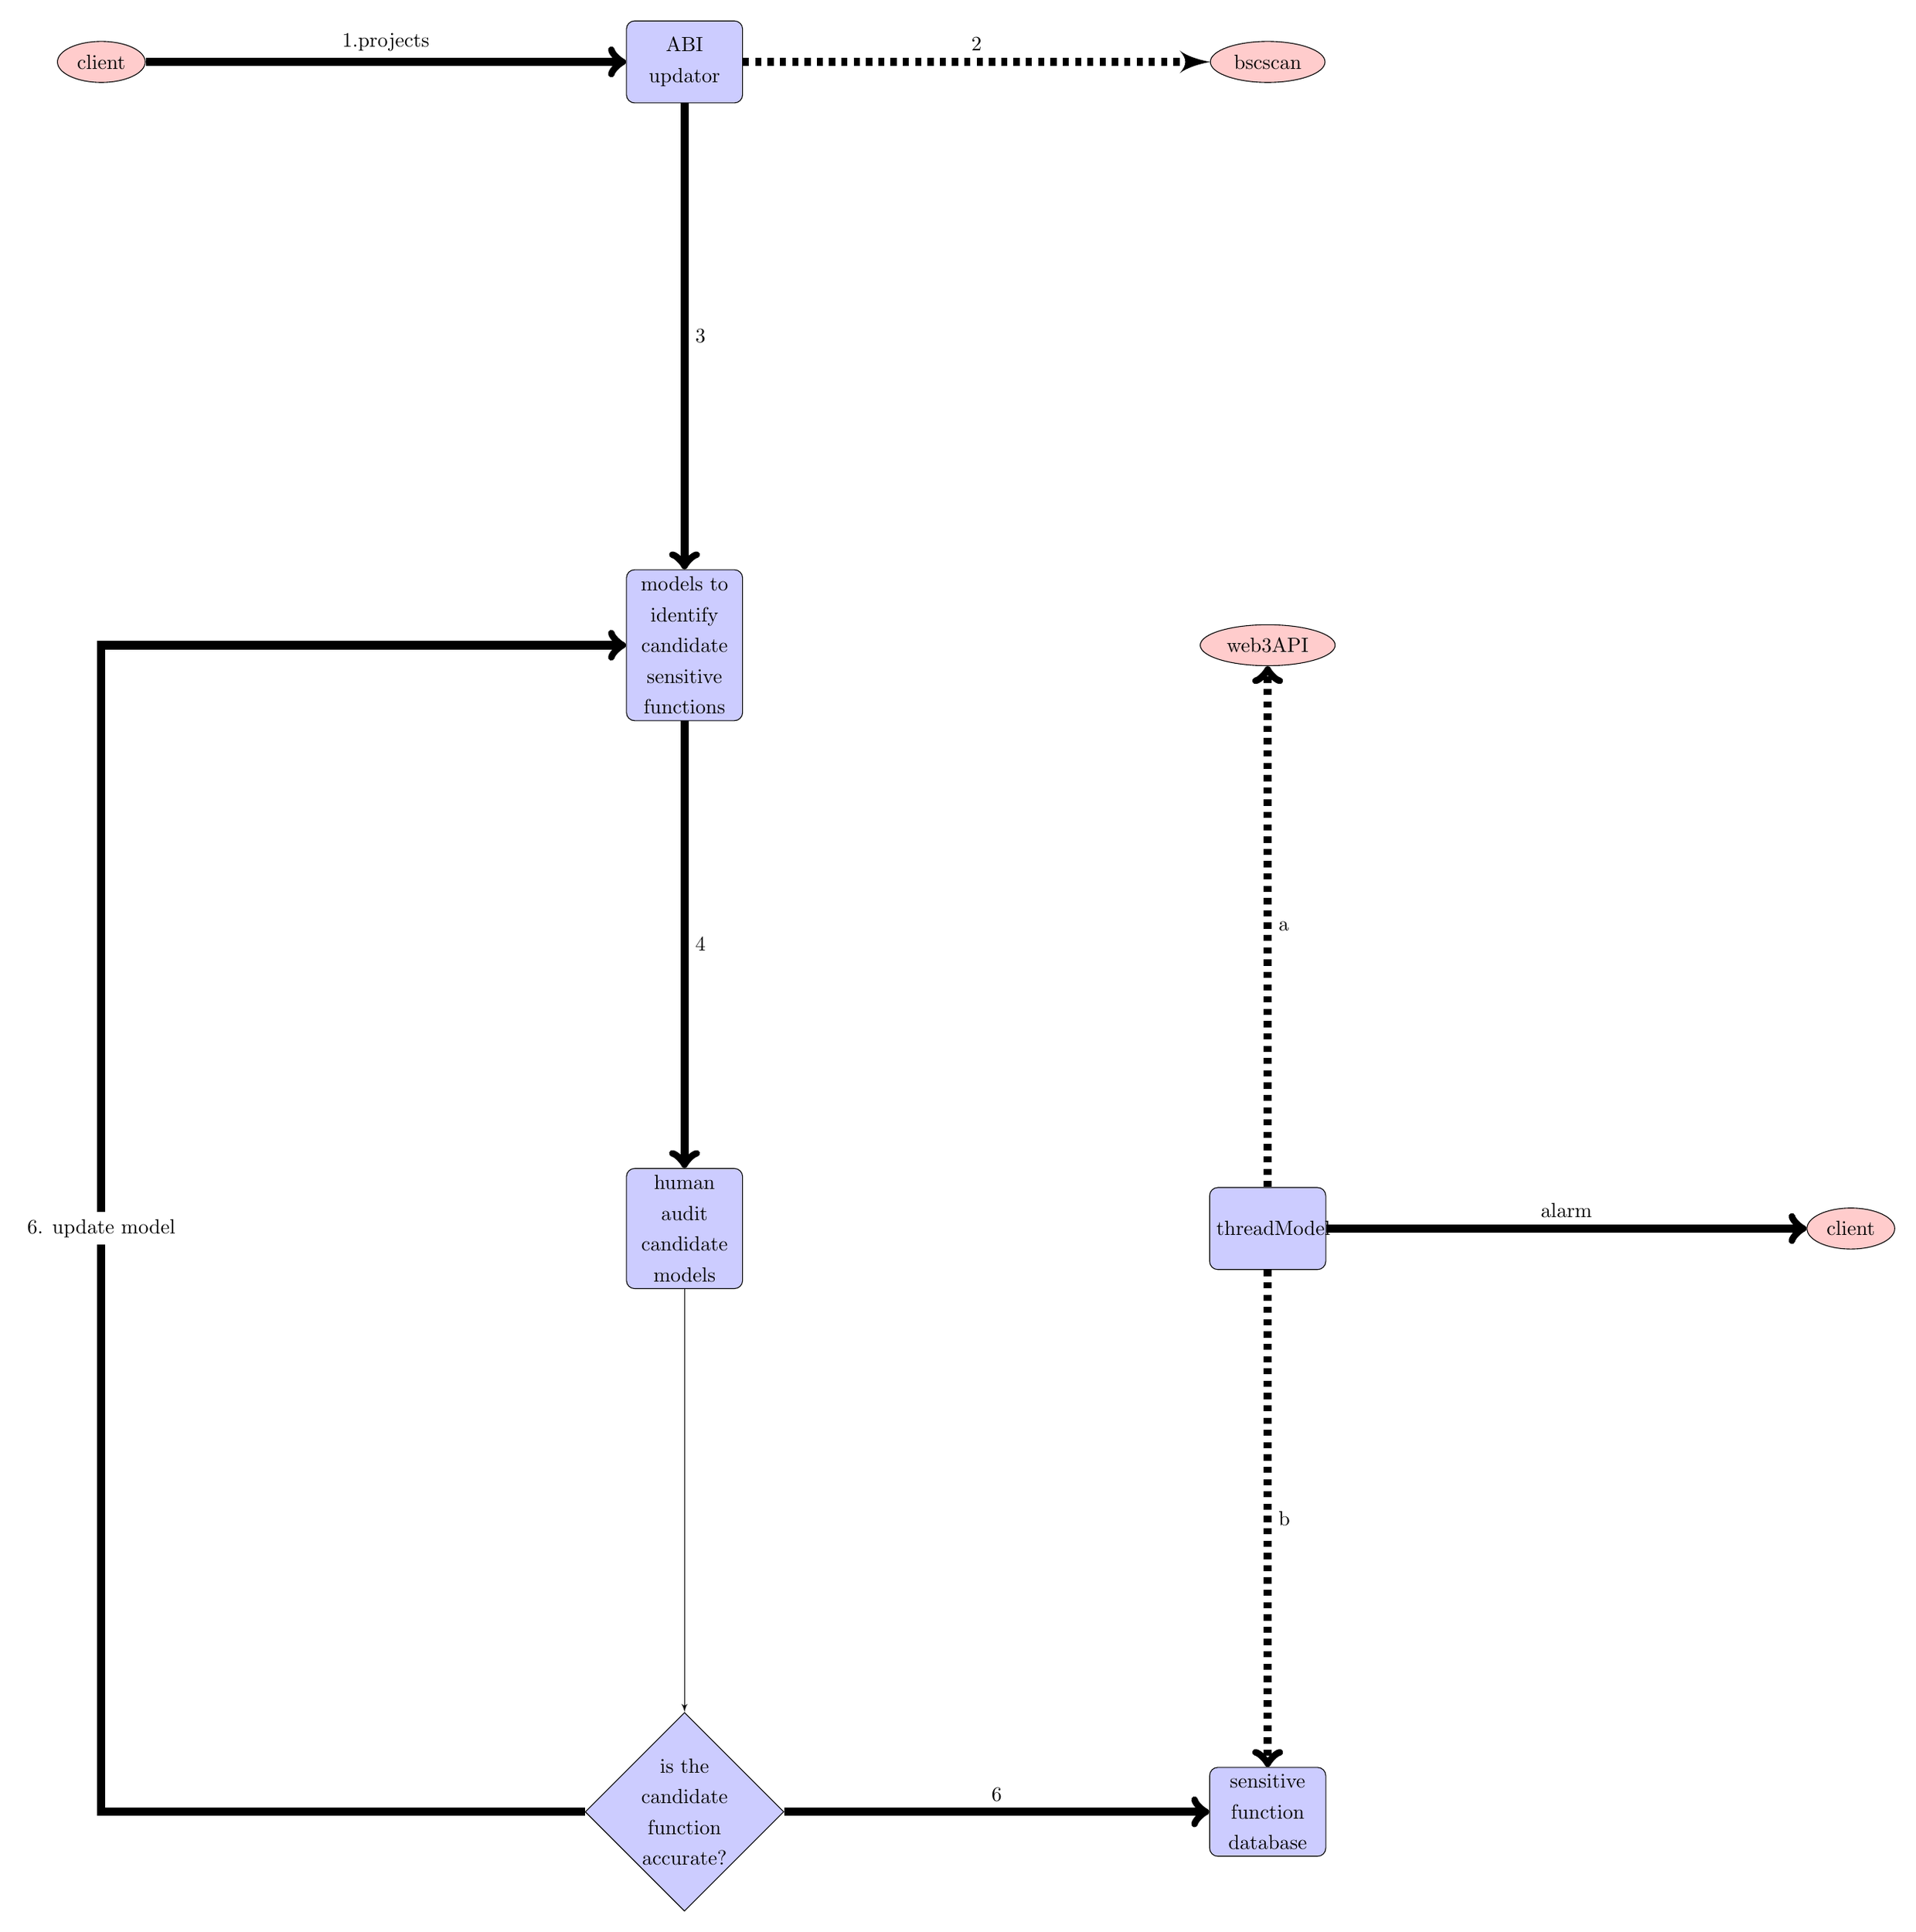
\begin{tikzpicture}[node distance = 10cm, auto]
    % Place nodes
    \node [block] (init) {ABI updator};
    \node [cloud, left of=init, node distance=10cm] (client1) {client};
    \node [cloud, right of=init, node distance=10cm] (bscscan) {bscscan};
    \node [block, below of=init] (identify) {models to identify candidate sensitive functions};
    \node [block, below of=identify] (evaluate) {human audit candidate models};
    \node [left of=evaluate, node distance=10cm] (update) {6. update model};
    \node [decision, below of=evaluate, node distance=10cm] (decide) {is the candidate function accurate?};
     \node [cloud, right of=identify, node distance=10cm] (web3API) {web3API};
    \node [block, right of=evaluate, node distance=10cm] (threadModel) {threadModel};
    \node [cloud, right of=threadModel, node distance=10cm] (client2) {client};
    \node [block, right of=decide, node distance=10cm] (sensitiveFunctionDatabase) {sensitive function database};
    % Draw edges
    \draw [->, line width=4pt] (client1) -- (init) node [midway,above] {1.projects}; 
    \draw [->,line,dashed, line width=4pt]  (init)--(bscscan)node [midway,above] {2};
    \draw [->, line width=4pt] (init) -- (identify) node [midway,right] {3};
    \draw [->, line width=4pt] (identify) -- (evaluate)node [midway,right] {4};
    \path [line] (evaluate) -- (decide);
    \draw [  line width=4pt] (decide) -| node [near start] {} (update);
    \draw [->, line width=4pt] (update) |- (identify);
    
    \draw [->, line width=4pt] (decide) -- (sensitiveFunctionDatabase)node [midway,above] {6};
    \draw [->, dashed, line width=4pt] (threadModel) -- (web3API)node [midway,right] {a};
    \draw [->, dashed, line width=4pt] (threadModel) -- (sensitiveFunctionDatabase)node [midway,right] {b};
    \draw[->, line width=4pt] (threadModel) --(client2)node[midway,above] {alarm};
\end{tikzpicture}
%----------------------------------------------------------------------------------------
%   CONCLUSIONS BOX
%----------------------------------------------------------------------------------------

%\section*{} % this dummy section draws a horizontal line above conclusions
\vspace{2cm}
\begin{tcolorbox}[width=0.95\linewidth,colback={binanceyellow},frame empty,boxsep=1cm]
\section{Conclusions}
\begin{itemize}
    \item Strengthen knowledge of EVM compilation and execution
    \item Cross-team cooperation
    \item Rules and modeling on figuring abnormal behaviors
    \item Binance Infrastructure and Mainstream available resources for monitoring
    \item Understanding of business from higher view
    \item Balance limited security resources on projects to achieve better ulitity


\end{itemize}
\end{tcolorbox}    

%----------------------------------------------------------------------------------------
%   FORTHCOMING RESEARCH
%----------------------------------------------------------------------------------------



\end{multicols}
\end{document}